\chapter{Results} \label{study_results}

This Chapter describes all the results gathered throughout the study in a per RQ basis. This approach increase the traceability of the findings within the report as suggested by Runeson et al. \cite{case_study_software_engineering} (Item 20 in Appendix \ref{checklist_for_case_studies}).

Furthermore, for each research question the following schema is used. Firstly, they contain results yielded by the thematic analysis performed on archival records. Subsequently, for each relevant theme, they report the validation results obtained through semi-structured interviews described in section \ref{sec:semi-structured_interviews} or, where possible, results obtained through quantitative metrics.

\section{Research Question 1}

As defined in the Introduction chapter, the goal of this Research Question is to evaluate which aspects of Source Code decay are applicable to the Test code. The first phase of the study inspected the available documentation and meta-documentation sources in order to define the most relevant problems that, subsequently, have been analyzed through with quantitive metrics and validated through semi structured Interviews.

The thematic analysis revealed the codes listed in Table \ref{tab:themes_rq1}. Furthermore, Fig. \ref{fig:rq1_sources} reports the number of mentions of such codes on a per source basis.



\begin{table}
\renewcommand{\arraystretch}{1.5}
\centering
\begin{tabular}{ c p{4.3cm} p{4.6cm}}
    
    \hline       
    {\large Global Theme} & {\large Organizing Theme} & {\large Codes}\\
    \hline
    
    \multirow{4}{*}{\parbox[t]{4.3cm}{
        Source code bad habits that also arise in Test code}
    } & \multirow{2}{*}{\parbox[t]{4.3cm}{Modularity related issues}}
        & Complex functions \\
        & & DRY violations\\ 
        & & God functions\\ \cline{2-3}
        
    & \multirow{2}{*}{\parbox[t]{4.6cm}{Line related issues}}
        & Complex statements \\
        & & Arity problems \\
    \hline
\end{tabular}
\caption{Themes and codes related to RQ1 extrapolated from qualitative sources}
\label{tab:themes_rq1}
\end{table}

\begin{figure}[!htbp]
    \centering
    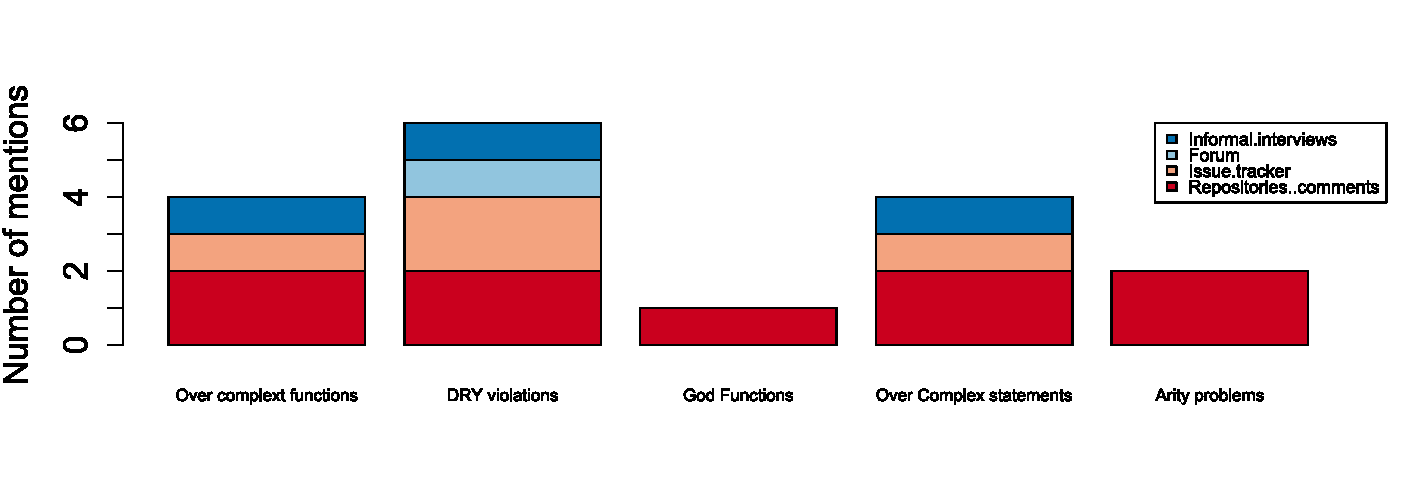
\includegraphics[width=\textwidth,keepaspectratio]{figure/results/rq1/sources.pdf}
    \caption{Codes with relatives Data sources for research question 1}
    \label{fig:rq1_sources}
\end{figure}


\subsection{DRY violations}
The DRY principle stands for \textit{``Don't Repeat Yourself''} and indicates the best practice of factoring out common logic in a separate entity to enhance code reuse.

Violation of this principle can be due several reasons and tends to greatly impact the maintainability efforts of the code base since a modification must be propagated throughout the code base a number of times equal to the number of copies of the logic interested.
    
\subsection{Function complexity}
The metric used to evaluate this Technical Debt Item is the well know cyclomatic complexity proposed by McCabe \cite{cyclomatic_complexity}.


    Figures \ref{fig:project_a_avg_complexity},\ref{fig:project_b_avg_complexity},\ref{fig:project_c_avg_complexity}, and \ref{fig:project_d_avg_complexity} display results generated by the process previously described in section \ref{sec:analysis_of_the_repos}.

    
\begin{figure}[!htbp]
    \centering
    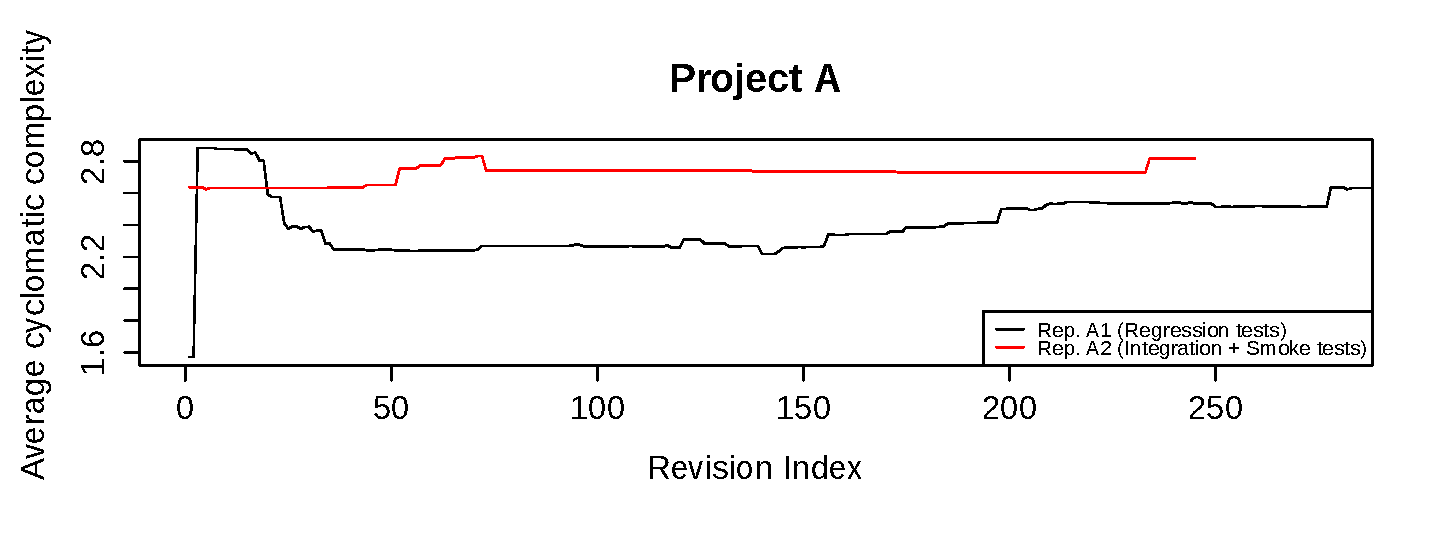
\includegraphics[width=\textwidth,keepaspectratio]{figure/results/rq1/project_a_avg_complexity.eps}
    \caption{Project A average cyclomatic complexity over time}
    \label{fig:project_a_avg_complexity}
\end{figure}

\begin{figure}[!htbp]
    \centering
    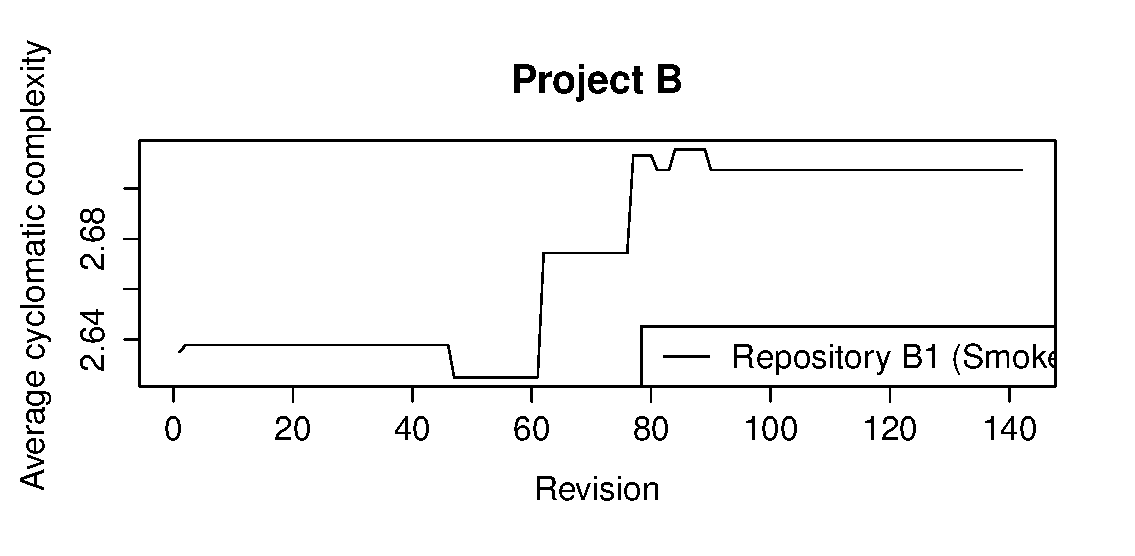
\includegraphics[width=\textwidth,keepaspectratio]{figure/results/rq1/project_b_avg_complexity.eps}
    \caption{Project B average cyclomatic complexity over time}
    \label{fig:project_b_avg_complexity}
\end{figure}

\begin{figure}[!htbp]
    \centering
    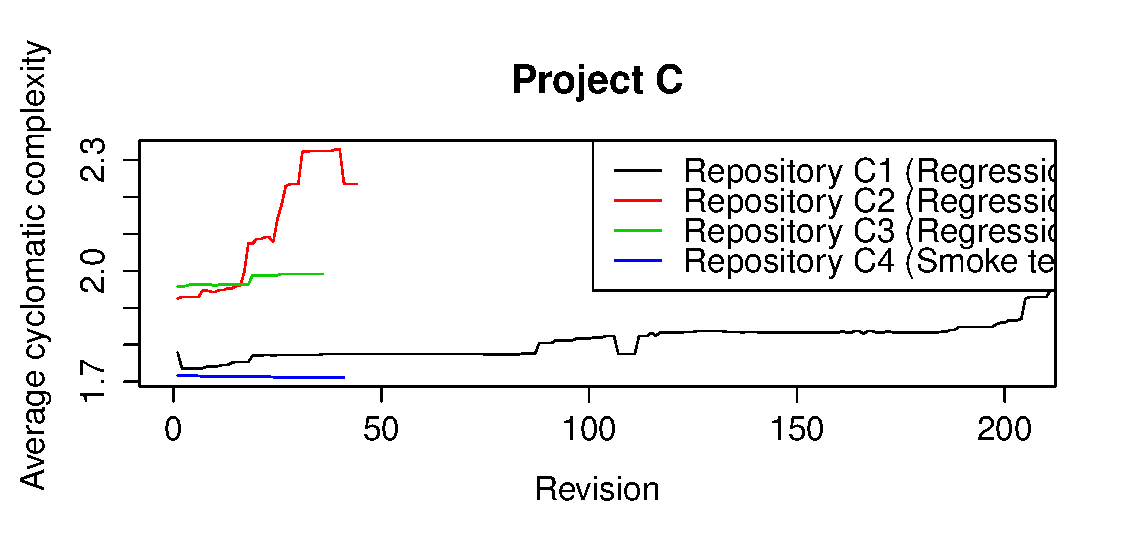
\includegraphics[width=\textwidth,keepaspectratio]{figure/results/rq1/project_c_avg_complexity.eps}
    \caption{Project C average cyclomatic complexity over time}
    \label{fig:project_c_avg_complexity}
\end{figure}

\begin{figure}[!htbp]
    \centering
    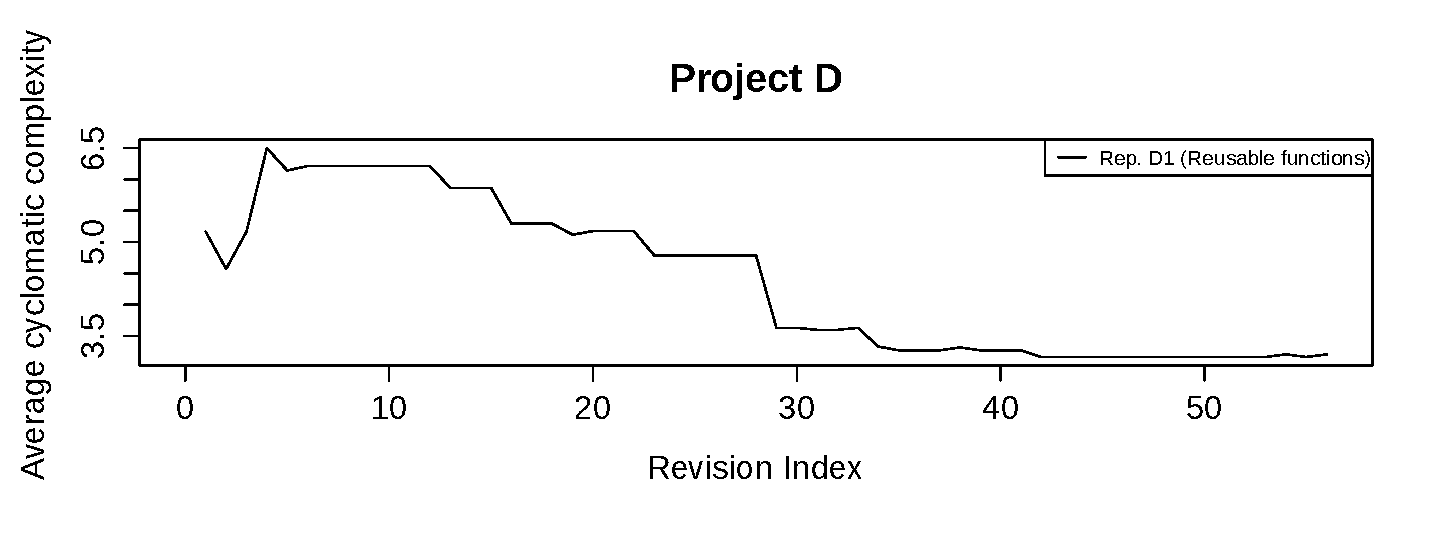
\includegraphics[width=\textwidth,keepaspectratio]{figure/results/rq1/project_d_avg_complexity.eps}
    \caption{Project D average cyclomatic complexity over time}
    \label{fig:project_d_avg_complexity}
\end{figure}

\FloatBarrier

\subsection{Complex statements}
This problem arises when the code includes statements that execute several operations at once. As steted by Stemlos et al. \cite{metrics_source_code}, a high number of such statements hinders understandability and readability of the code base.

A common accepted threshold is based on the number of characters used in a line. A number greater that eighty is considered too high and hence must be indented or the statement should be broken down in several sub-statements.

\begin{figure}[!htbp]
    \centering
    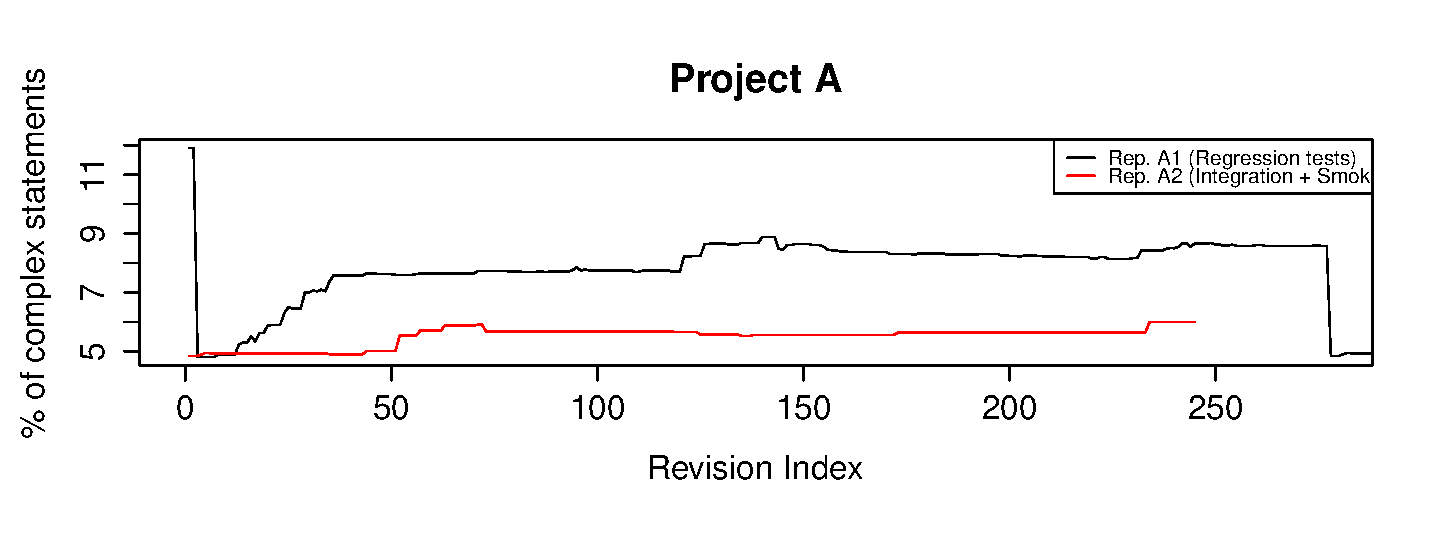
\includegraphics[width=\textwidth]{figure/results/rq1/statement_complexity_project_a.eps}
    \caption{Project A percentage of complex statements}
    \label{fig:statement_complexity_project_a}
\end{figure}

\begin{figure}[!htbp]
    \centering
    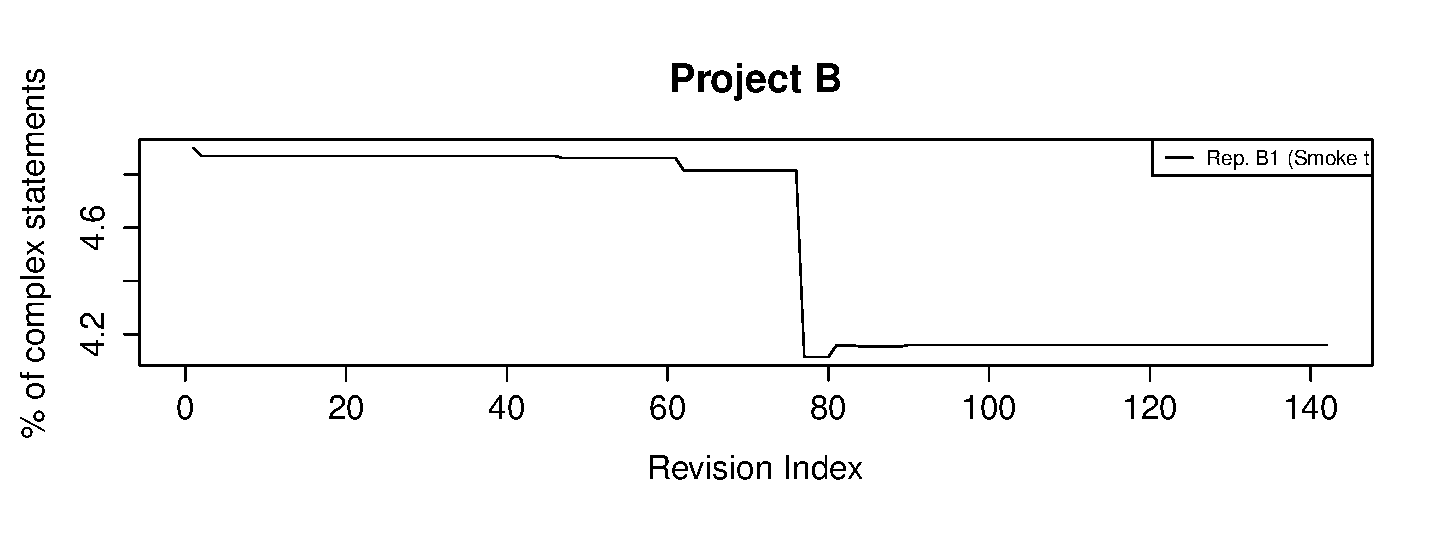
\includegraphics[width=\textwidth]{figure/results/rq1/statement_complexity_project_b.eps}
    \caption{Project B percentage of complex statements}
    \label{fig:statement_complexity_project_b}
\end{figure}

\begin{figure}[!htbp]
    \centering
    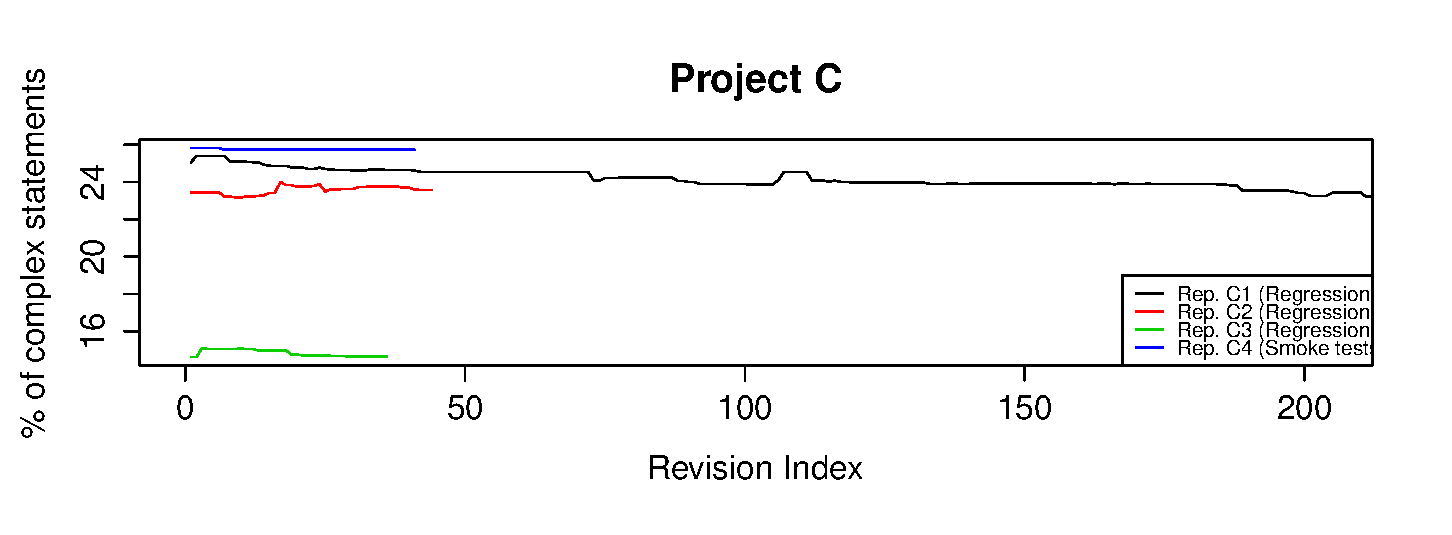
\includegraphics[width=\textwidth]{figure/results/rq1/statement_complexity_project_c.eps}
    \caption{Project C percentage of complex statements}
    \label{fig:statement_complexity_project_c}
\end{figure}

\begin{figure}[!htbp]
    \centering
    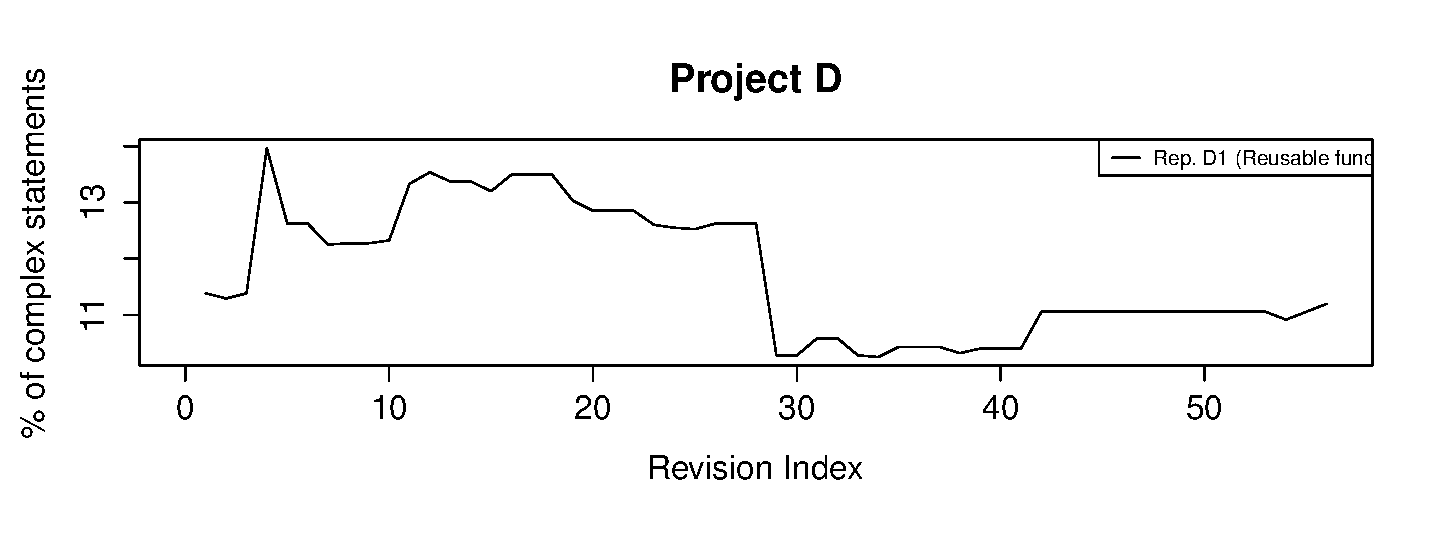
\includegraphics[width=\textwidth]{figure/results/rq1/statement_complexity_project_d.eps}
    \caption{Project D percentage of complex statements}
    \label{fig:statement_complexity_project_d}
\end{figure}


\section{Research Question 2}

The scope of User Interface tests is to validate the state of the User Interface after a predefined series of actions occurred. However, this entails a different use for the constructs compared to conventional source code and possibly new ones specific for these use cases. For this reason the second RQ will inspect these unique items.

However, keeping into account the differences between property based testing and image recognition testing is important. The former uses property or meta-properties of UI components to identify them and simulate user events over them. The latter, instead, uses image recognition algorithms to identify such widgets. This different identification method imposes different approached when creating the test suite that are analyzed separately in the following sections, presenting both quantitative and qualitative results.


  
\begin{table}
\renewcommand{\arraystretch}{1.5}
\centering
\begin{tabular}{ c p{4.3cm} p{4.6cm}}
    
    \hline       
    {\large Global Theme} & {\large Organizing Theme} & {\large Codes}\\
    \hline
    
    \multirow{7}{*}{\parbox[b]{4.3cm}{
        User interface testware specific issues
    }
    } & \multirow{4}{*}{\parbox[c]{4.3cm}{Image recognition problems}}
        & Too sensitive \\
        & & False positive and negative results\\
        & & Not reusable\\ 
        & & Not suitable for responsive environments (e.g. web applications)\\ \cline{2-3}
        
    & Property based problems & Impossible to foresee when it will break\\ \cline{2-3}
        
    & Coordinated based problems  & Too fragile\\ \cline{2-3}
        
    & UFT specific problems & Based on binary files\\
        
    \hline
\end{tabular}
\caption{Themes and codes related to RQ1 extrapolated from qualitative sources}
\label{tab:themes_rq2}
\end{table}

\begin{figure}[!htbp]
    \centering
    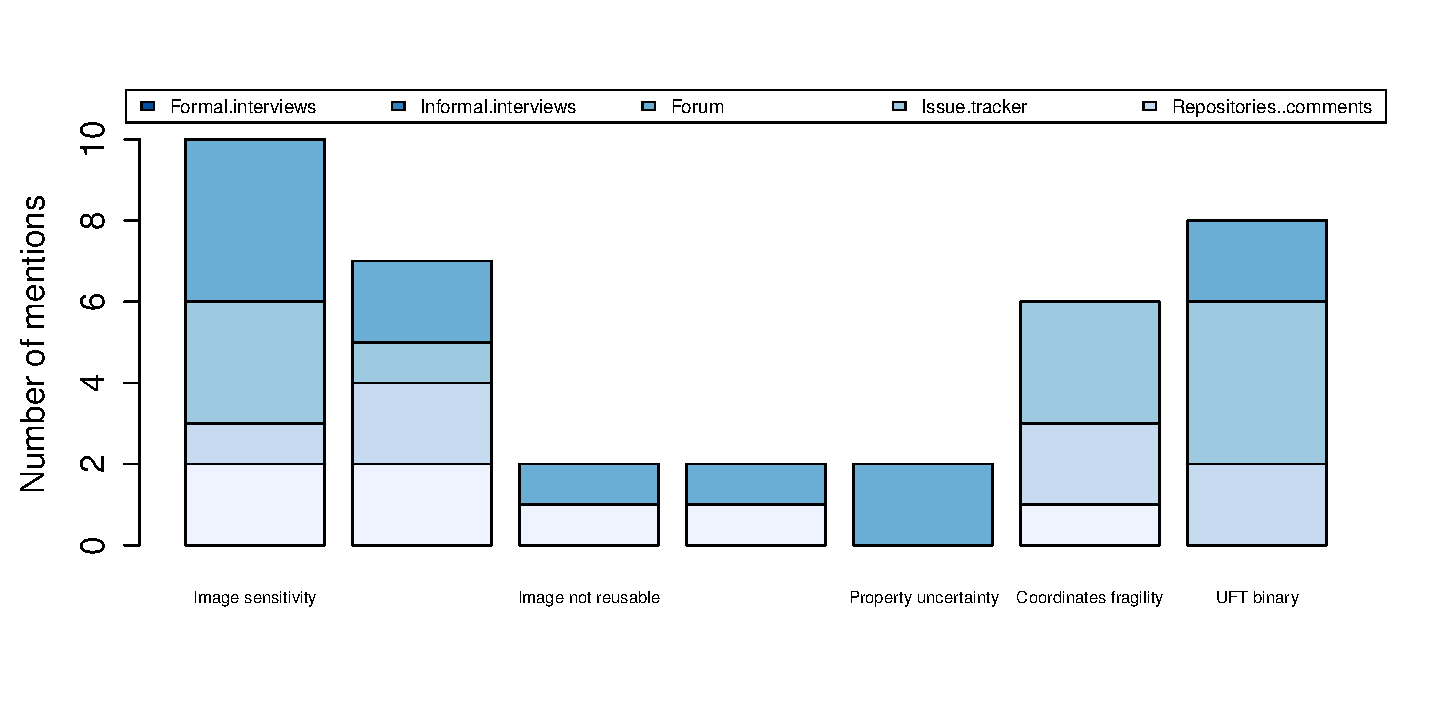
\includegraphics[width=\textwidth,keepaspectratio]{figure/results/rq2/sources.eps}
    \caption{Codes with relatives Data sources for research question 2}
    \label{fig:rq2_sources}
\end{figure}


\section{Research Question 3}

Finally, the purpose of this RQ is to complete the description of the TD items identified by RQ 1 and RQ 2. Once again, qualitative and quantitative data has been treated separately.

\subsection{Qualitative Data}
    

\subsection{Quantitative Data}
    

